In order to evaluate our model we ran experiments over three corpus to compare the typical LDA and his formulation with Boojum prior . We used a 20 news groups dataset, a nips 2012 set of articles and a the reuter50 corpus. Each of them were divided into a training and test set corpus with a ratio 80-20 percent respectively. We fit both a classical LDA model and the extented LDA using the training set. The test set was used to assert to convergence of the training phase by computing the perplexity of the model. To compute it we follow a fold-in procedure and  use the approximation in (Asuncion, 2009) to compute the perplexity. Hence the topic-word distribution is fit on the learning set and the document-topic distribution is evaluated on the testing set, thus the perplexity of the model is computed as follow: 
\[
\begin{array}{l@{\hspace{.3cm}}l}
\log p(x^{test}) = \sum_{dw} N_{dw} \log \sum_k \hat{\theta}_{kd} \hat{\phi}_{wk} \\
perplexity(x^{test}) = \exp(- \frac{\log p(x^{test})}{\sum_d N_d})
\end{array}
\]
%$N_{dw}$ being the count of word in each document. This approximation of the perplexity , which is not directy computable, is approximed by a lower bound given by the Jensen inequality. ~\\
In the given settings we experienced the Boojum on different combinations. We tried to infer the model with this conjugate prior for the 3-case possibility namely:
\begin{itemize}
\item on the topic-word distribution only with classical Newtows optimization for $\alpha$,
\item on the document-topic distribution only,
\item on both distributions. 
\end{itemize}
We found that using constant asymmetric prior on the document-topics distribution and a boojum for the topic-words one was more efficient in term of perplexity.
% Discussion here for the contradiction with Wallach ?

We compared then the perplexity on several subset of training and testing and for various values of $K$, the number of topics. In figure \ref{fig:pp_D} we compute the ratio of perplexity to the two model. It shows a light tendancy of the model to be better for smaller corpora and to approach LDA performance when it increases. This is especially true for the 20 news group corpora, who maybe fit the assumptions behind the boojum in term of how his features are distributed. 

\begin{figure}[h]
\label{fig:pp_D}
%\vspace{.3in}
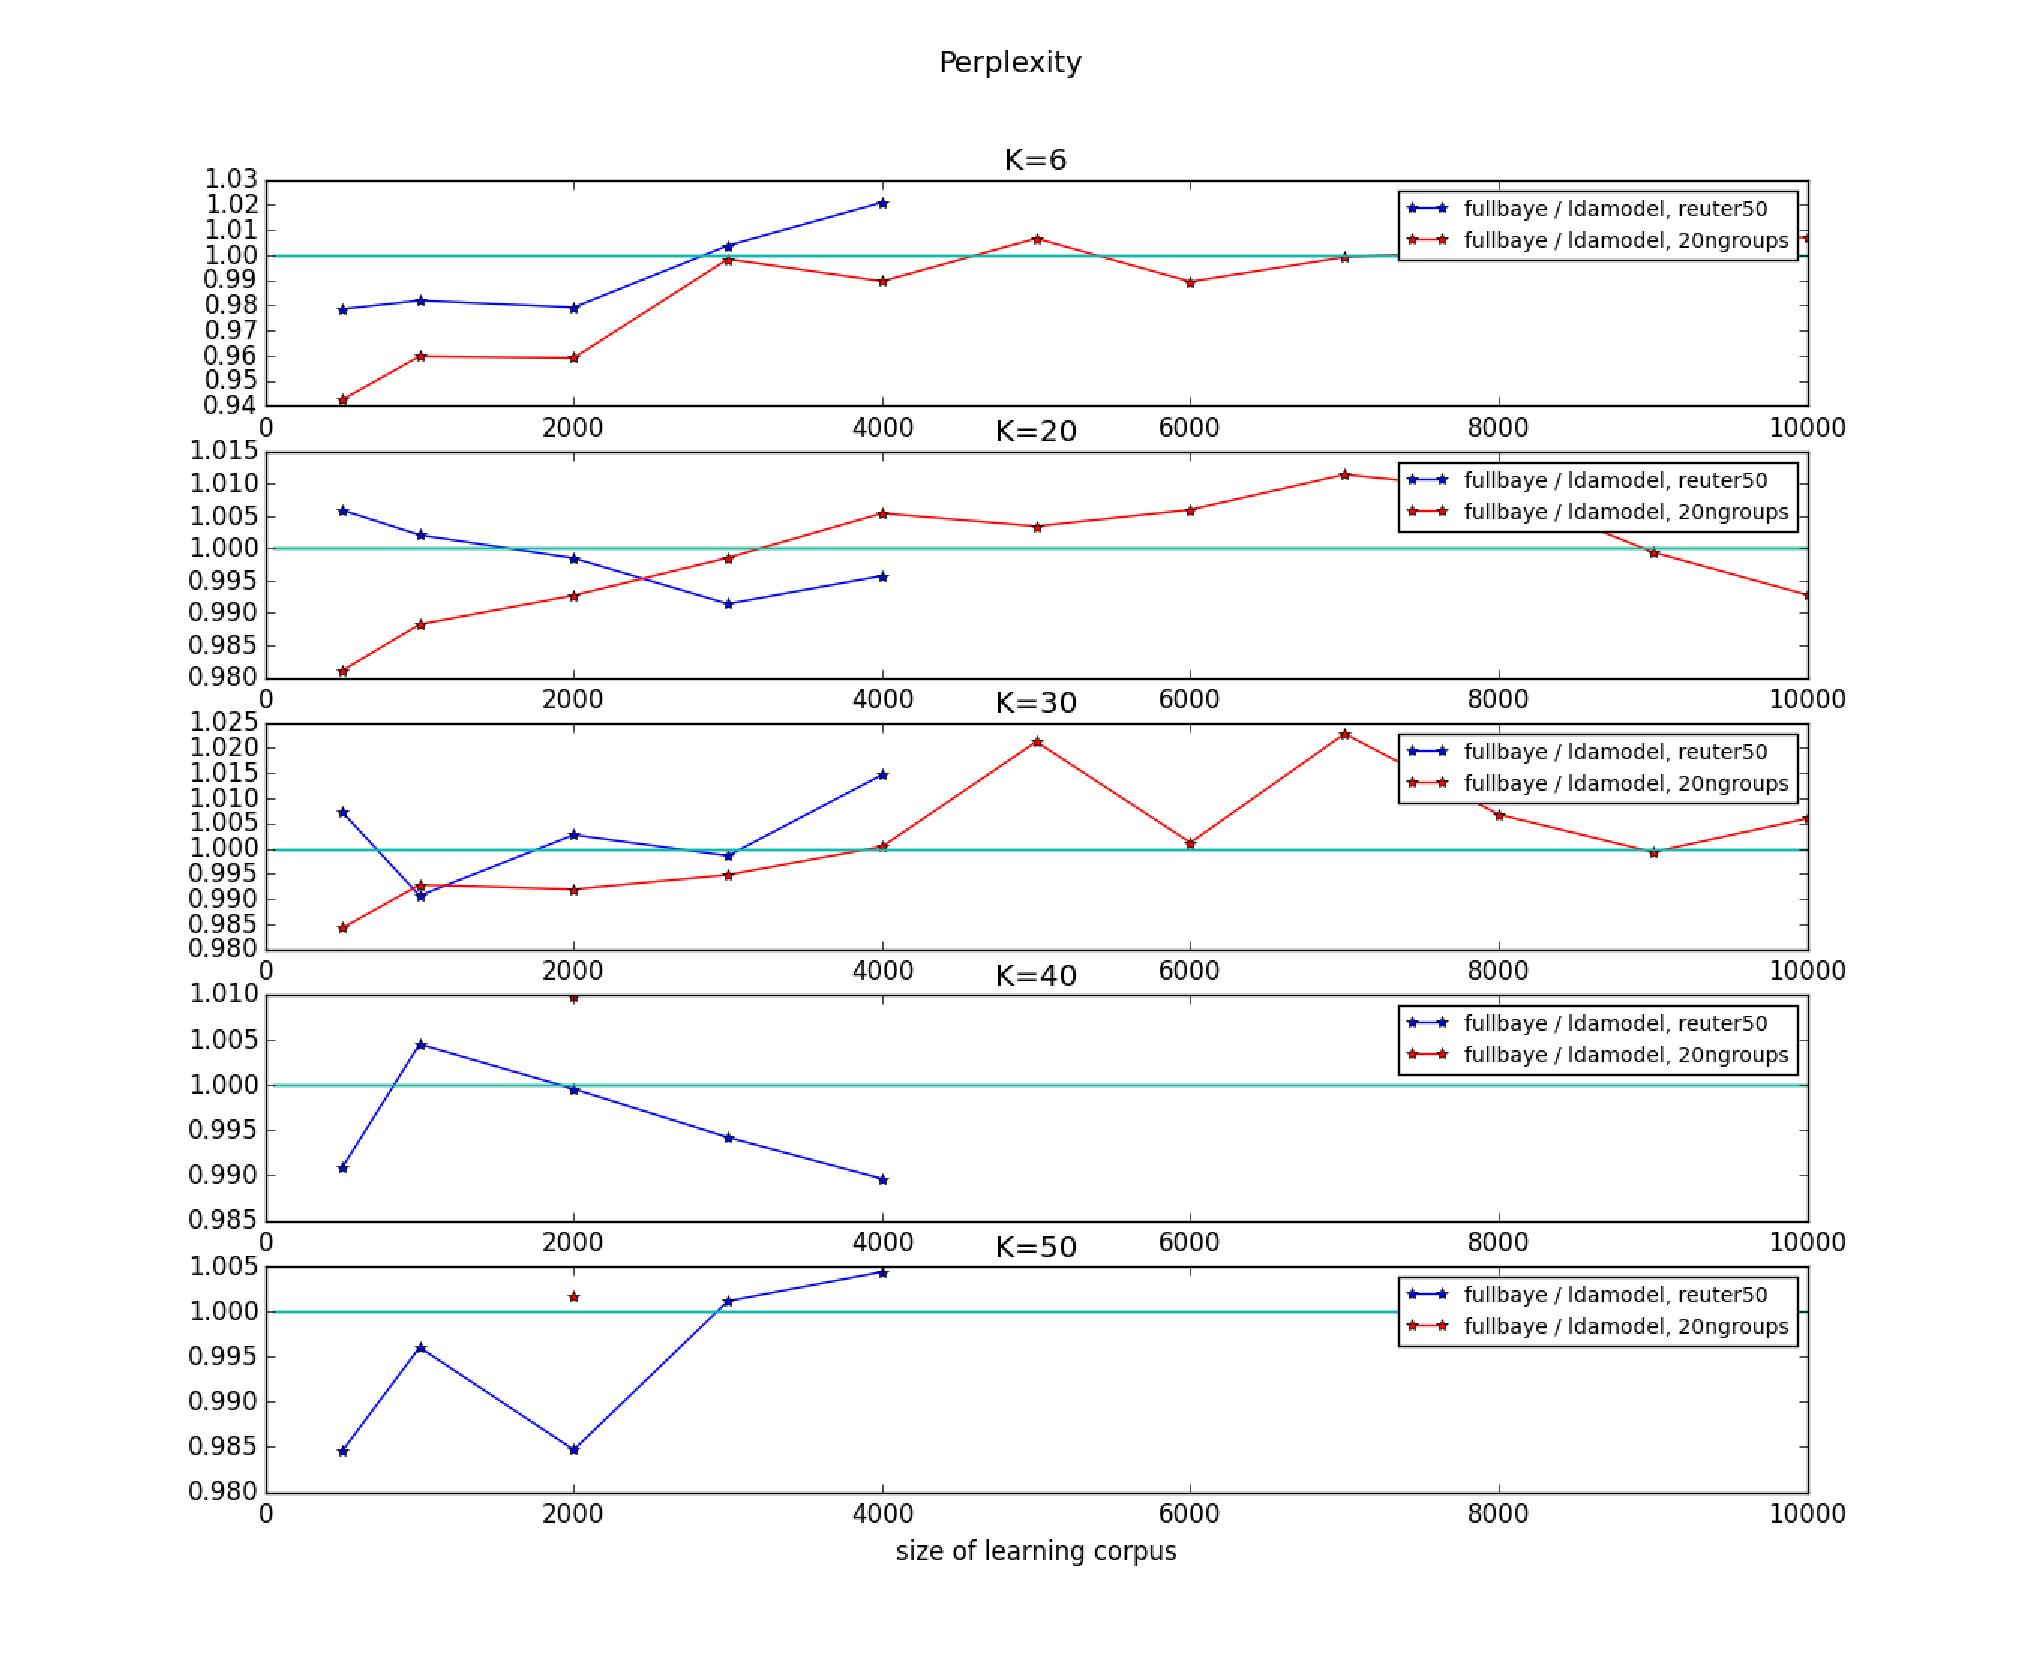
\includegraphics[width=9cm, height=14cm]{results/pp_D.eps}
%\vspace{.3in}
\caption{Ratio of perplexity of boojum LDA over classical LDA on several size of dataset and for different number of topic}
\end{figure}

The figure \ref{fig:pp_conv}, show a particular case of leaning convergence for the 20 news group. We can see that the our model converge better and faster than LDA in this case. 

\begin{figure}[h]
\label{fig:pp_conv}
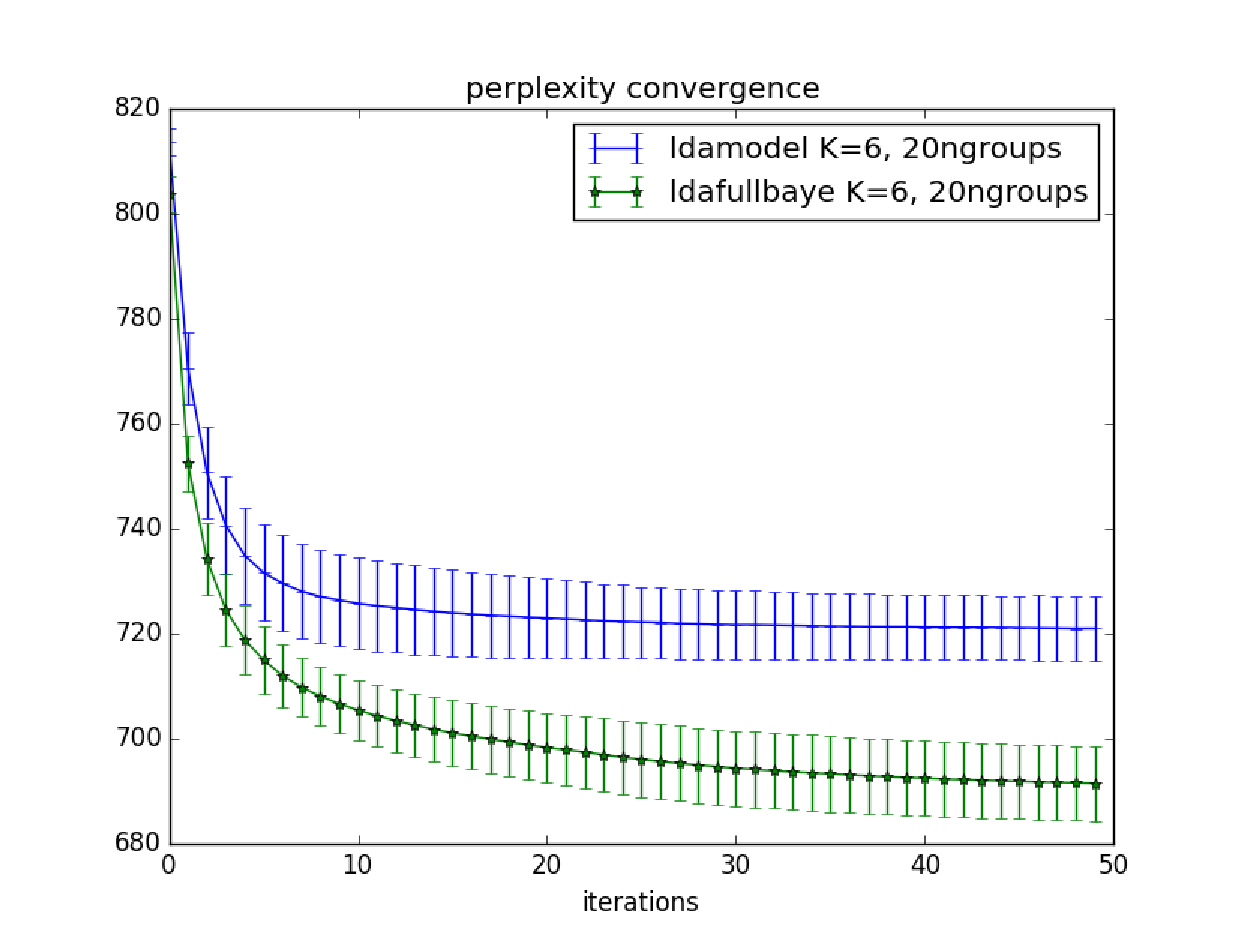
\includegraphics[scale=0.4]{results/pp_conv.eps}
\caption{Result of perplecity on testing set at each iterations of the variationnal bayes iteratino for the 20 news group corpus}
\end{figure}

Finally, the complexity of the update for the boojum in this case add no complexity compared to LDA fitting as suggested in figure \ref{fig:time}

\begin{figure}[h]
\label{fig:time}
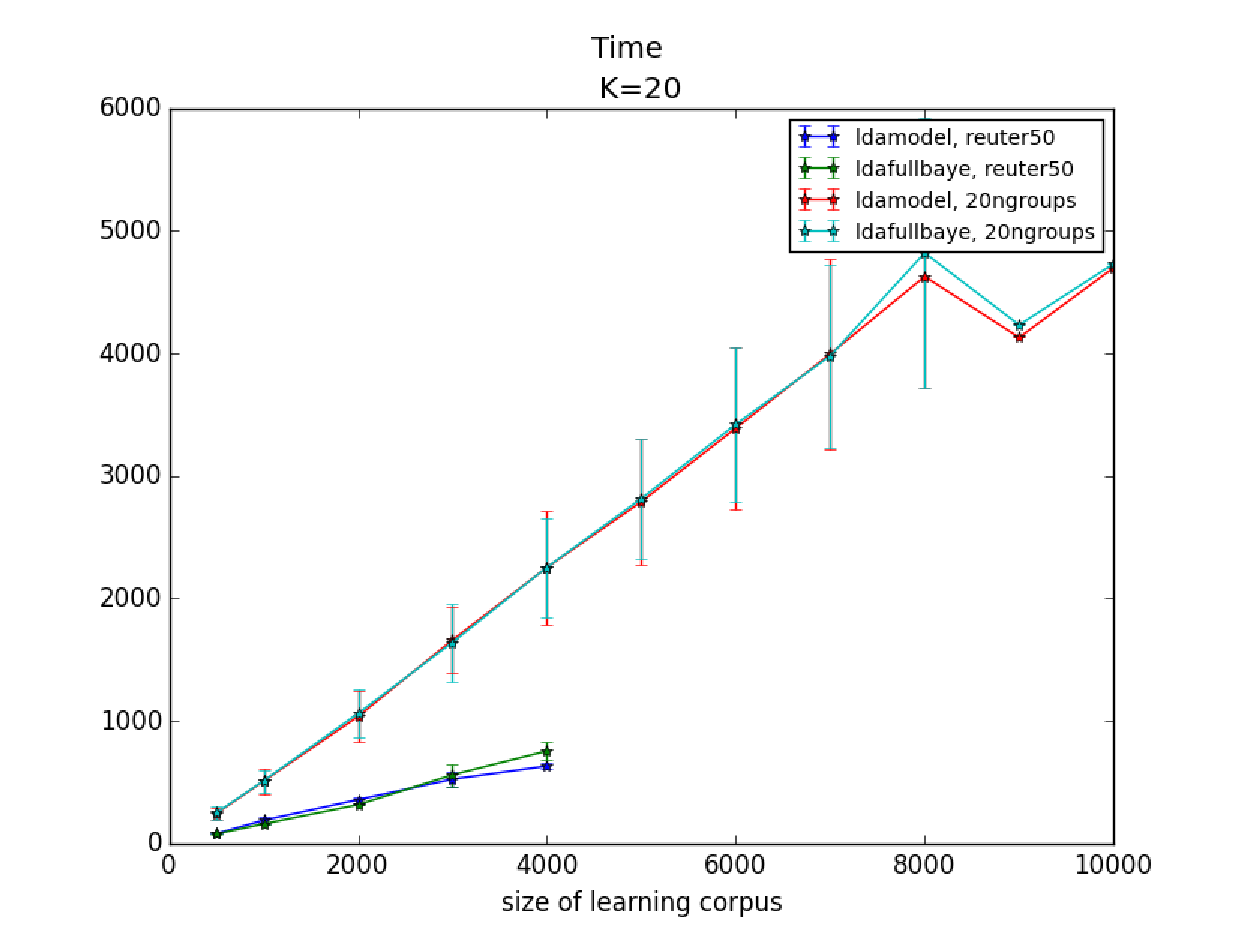
\includegraphics[scale=0.4]{results/time.eps}
\caption{Time of inference for 50 iterations of variational bayes.}
\end{figure}

\begin{figure}[h]
\label{fig:pp_K}
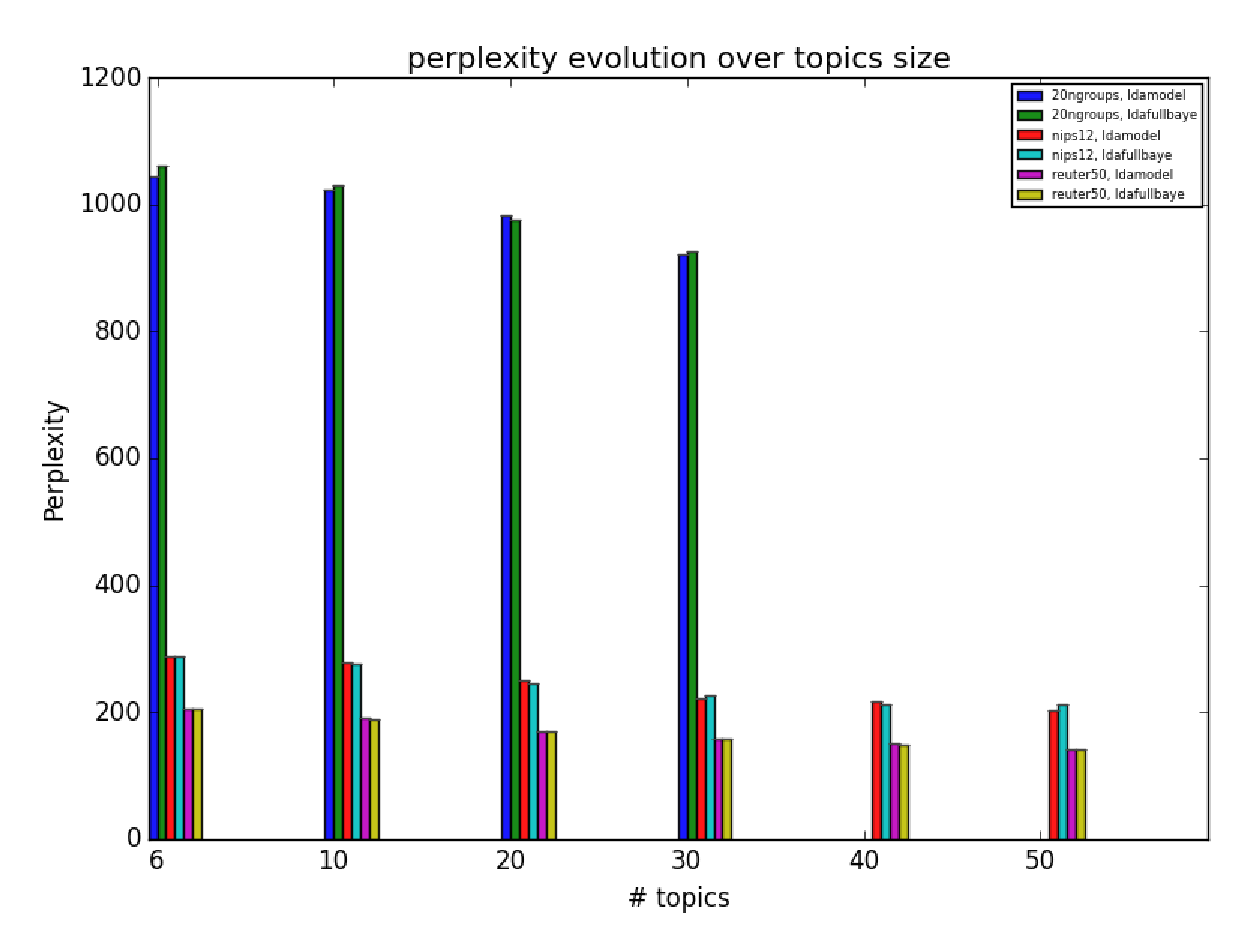
\includegraphics[scale=0.4]{results/pp_K.eps}
\caption{For several number of topic, we show the perplexity of all the corpus for the classical LDA and the boojum extension.}
\end{figure}

%Each inference procedure was run over 50 iterations and reproduced 10 times to provide a stability measure. Therefore, the figure shows the mean perplexity for each run and his variance.
